\documentclass[tikz, border=2pt]{standalone}
\usepackage{graphicx} 
\usepackage{tikz} 
\usepackage{tikz-3dplot} 
\usetikzlibrary{angles,quotes,arrows.meta, positioning} 
\usepackage{pgfplots} 
\pgfplotsset{compat=1.18} % Pacchetti Matematici 
\usepackage{amsmath, amssymb, amsthm} 

\definecolor{myblue}{HTML}{139FE9}
\begin{document}
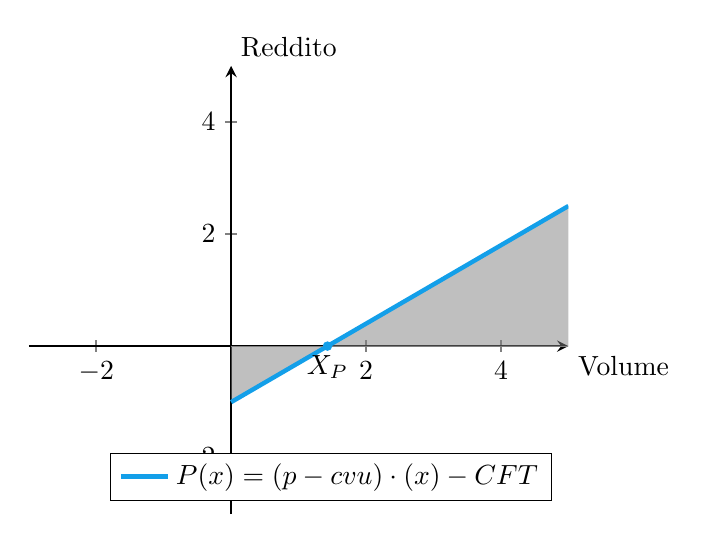
\begin{tikzpicture}[scale = 1,
            declare function={
                    f(\x) = (1.5-0.8)*\x - 1;
                    g(\x) = 0;
                }]
        \def\p{1.428}
        \begin{axis}
            [
                xlabel={\( \text{Volume} \)},
                ylabel={\( \text{Reddito} \)},
                xmin=-3, xmax=5,
                ymin=-3, ymax=5,
                grid=both,
                grid=both,
                grid=none, axis lines=middle, 
                axis line style={-stealth, thick},
                tick style={thick},
                xlabel style={at={(ticklabel* cs:1)}, anchor=north west},
                ylabel style={at={(ticklabel* cs:1)}, anchor=south west},
                samples=100, unbounded coords=jump, legend pos=south east
            ]
            \coordinate (A) at (axis cs:\p,{f(\p)});
            \coordinate (B) at (axis cs:5,{f(5)});
            \coordinate (C) at (axis cs:5,{g(5)});
            \coordinate (D) at (axis cs: 0,{f(0)});
            \coordinate (E) at (axis cs: 0,{g(0)});
            \fill[gray, opacity=0.5] (A) -- (B) -- (C) -- cycle;
            \fill[gray, opacity=0.5] (A) -- (D) -- (E) -- cycle;
            \addplot[domain=0:5, ultra thick, smooth, color=myblue]{f(x)};
            \addplot[domain=0:5, ultra thin, smooth, color=gray]{g(x)};
            \draw [dashed, thick, color=gray] (axis cs: \p, {f(\p)}) -- (axis cs: \p, 0);
            \filldraw[color=myblue] (axis cs: \p, {f(\p)}) circle (1.5pt);
            \node[below] at (axis cs: \p, 0) {\(X_P\)};
            \legend{$P(x) = (p - cvu) \cdot (x) - CFT$}
        \end{axis}
    \end{tikzpicture}
\end{document}